% !TeX root = ../thuthesis-example.tex
\chapter{Background and related works}\label{chapter-2}
In this chapter, we introduce the relevant background (Section \ref{background}) and related works (Section \ref{related-works}). 

\section{Background}\label{background}
Our inference system is designed primarily for serving GPT-based MoE models. In this section, we discuss the components of a typical GPT-MoE architecture, starting from the underlying transformer architecture (Section \ref{transformer}), the GPT architecture and how it differs from the original transfomer model (Section \ref{gpt-overview}), the MoE layer (Section \ref{moe-layer}), and finally how GPT models can be \textit{MoEfied} to effectively incorporate MoE layers (Section \ref{gpt-moe}).

\subsection{Transformer}\label{transformer}
The transformer architecture is a type of neural network architecture that was introduced in 2017 by Vaswani et al.~\cite{transformer} It was primarily designed for natural language processing (NLP) tasks such as language modeling, machine translation, or text summarization. Since then, transformers have become the most popular architecture in deep learning, and they have been adapted for media types other than text, for example images~\cite{vit}, audio~\cite{wav2vec}, and video~\cite{vivit}.

The key component in the transformer architecture is the self-attention module, which allows the model to take into account the context of a given token by weighing the relevance of different parts of the input sequence while processing it. During the training phase, when the context both before and after the current word is available, a transformer may use a bidirectional attention. During inference, on the other hand, the transfomer uses a causal attention mechanism to only consider the previous tokens as the context for the current word. Compared to previous NLP architectures such as convolutional neural networks (CNNs) or recurrent neural networks (RNNs), the transformer architecture has the advantage that it does not require the sequential processing of input tokens. This opens up opportunities for parallel implementation, which translate to better performance. 

The transformer architecture (see Figure \ref{fig:original-transformer}) consists of an encoder and a decoder, each composed of multiple layers of identical sub-modules. The encoder takes an input sequence and generates a hidden representation of the sequence, while the decoder takes the hidden representation and generates an output sequence.

\begin{figure}[H]
    \centering
    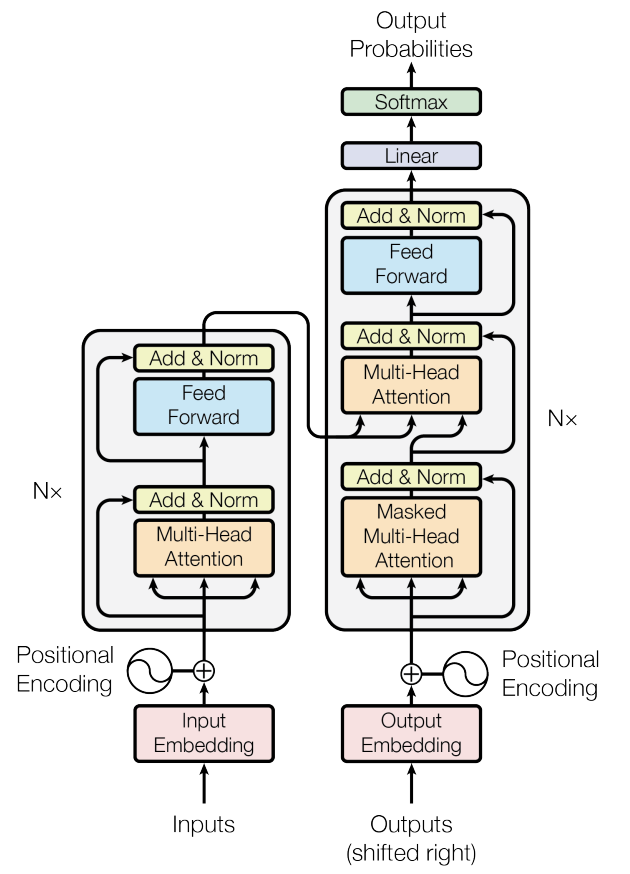
\includegraphics[width=0.6\linewidth]{figures/transformer-architecture.png}
    \caption{\textbf{The Transformer architecture}. The illustration~\cite{transformer} shows the original Transformer architecture, with both the encoder and the decoder modules, featuring the multihead-attention operator}
    \label{fig:original-transformer}
\end{figure}

Each layer in the transformer architecture contains two types of sub-modules: the multi-head attention module (see Figure \ref{fig:mha}) and the feedforward neural network. The encoder layer only has a single attention sub-module, whereas the decoder contains two, unless the model is a decoder-only model. The multi-head attention module computes a weighted average of the input sequence, where the weights are determined by the attention mechanism. The attention mechanism computes the similarity between each token in the input sequence and every other token, and uses these similarities to compute a set of attention weights. These weights are used to compute a weighted average of the input sequence, where the weights reflect the importance of each token in the sequence. The feedforward neural network applies a linear transformation to the input sequence, followed by a non-linear activation function such as ReLU. Finally, a layer normalization is applied to the output of the attention, and a residual connection is added. The transformer architecture also includes positional encoding, which allows the model to distinguish between tokens based on their position in the sequence. The positional encoding is added to the input embeddings before they are processed by the decoder.

\begin{figure}[H]
    \centering
    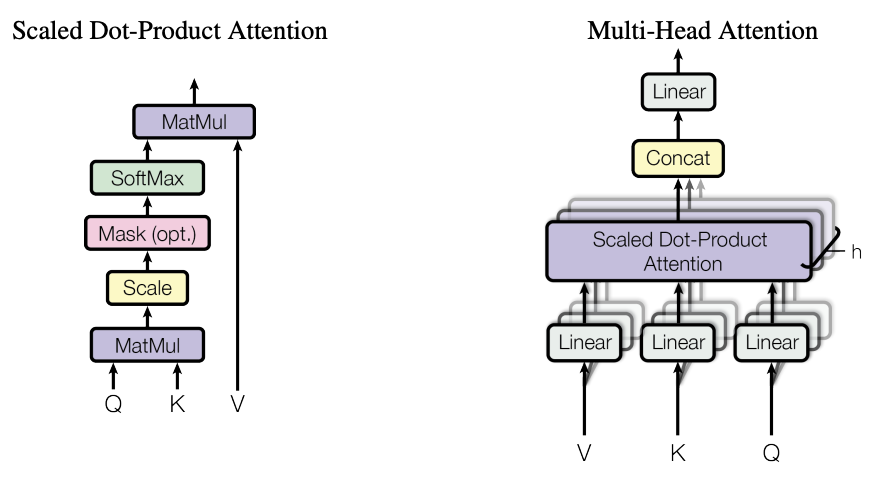
\includegraphics[width=0.6\linewidth]{figures/mha_architecture.png}
    \caption{\textbf{The Multihead Attention operator ~\cite{transformer}}}
    \label{fig:mha}
\end{figure}

\subsection{GPT models}\label{gpt-overview}
\begin{figure}[H]
    \centering
    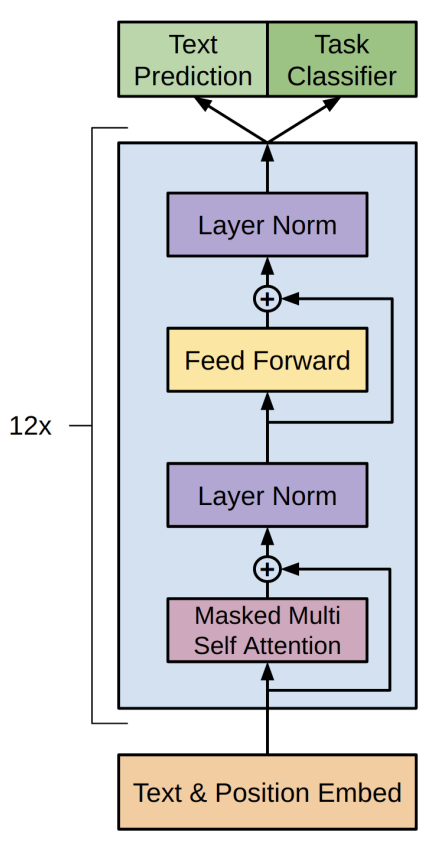
\includegraphics[width=0.3\linewidth]{figures/gpt1_architecture.png}
    \caption{\textbf{The GPT architecture}. The illustration ~\cite{gpt1} shows the original GPT architecture. GPT-2 and GPT-3 use the same architecture, with very small modifications }
    \label{fig:gpt-original}
\end{figure}
A typical GPT architecture is shown in Figure \ref{fig:gpt-original}.
The GPT architecture~\cite{gpt1, gpt2} differs from a plain Transformer architecture in a few ways. Overall, the main difference is that GPT models are decoders-only, meaning that they only employ the decoder layers from the transformer, and do not use the encoder layers. In addition to dropping the encoder layers, the GPT has the following characteristics:
\begin{itemize}
    \item \underline{Unidirectional attention}: The original Transformer architecture is bidirectional, meaning that it takes into account both past and future tokens when encoding a sequence of text. The GPT architecture, on the other hand, is unidirectional and only considers the past tokens when generating output.
    \item \underline{Causal Masking}: The original Transformer architecture is only required to use masking to prevent the model from attending to future tokens during inference, whereas the GPT architecture uses masking to prevent the model from attending to any tokens beyond the current one during both training and inference.
    \item \underline{Positional Encoding}: The GPT architecture uses a slightly different method of positional encoding compared to the original Transformer architecture. In GPT, the positional encoding is added directly to the input embeddings, whereas in the original Transformer architecture, the positional encoding is added to the output of the multi-head attention layer.
    \item \underline{Training tasks}: The pre-training objectives used for the GPT architecture are different from the original Transformer. Specifically, GPT is pre-trained using a language modeling objective, where the model is trained to predict the next token in a sequence, while the original Transformer is pre-trained using a masked language modeling objective, where the model is trained to predict masked tokens in a sequence.
\end{itemize}

Overall, the GPT architecture is a modification of the Transformer architecture, tailored specifically for language generation tasks such as text completion and dialogue generation. The differences in architecture and pre-training objectives are designed to make the model better suited to these tasks, resulting in state-of-the-art performance on a variety of natural language generation benchmarks.

\subsection{Mixture of Experts}\label{moe-layer}
A Mixture-of-Experts (MoE) layer, whose structure can be seen in Figure \ref{fig:moe-illustation}, combines a set of \textit{experts} with a \textit{gating network} (also called \textit{routing network}). Each expert is usually a feed-forward neural network (FFN), and the gating network is a function routing each input token to a sparse subset of the experts. Through training of the gating network, different experts will thus end up specializing on different subsets of the input data. The dynamic nature of the MoE architecture comes from two main sources. First, tokens are not distributed equally among experts (although MoE models tend to use loss terms to prevent excessive load imbalance) due to the use of the gating function. In Figure \ref{fig:expert_popularity}, for example, we can see how the popularity of various experts changes over the course of the training iterations. Second, in many MoE models, the \textit{capacity factor} is adjusted dynamically during training \cite{switch_transformer, tutel, dynamoe}, resulting in additional changes to the execution plan.
\begin{figure}[H]
    \centering
    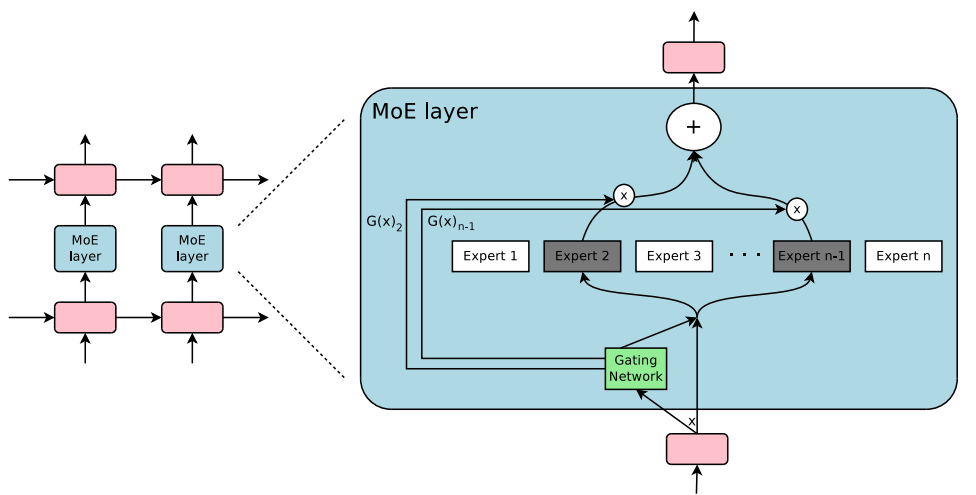
\includegraphics[width=0.6\linewidth]{figures/moe-illustration.png}
    \caption{\textbf{The Mixture of Expers (MoE) architecture}. The illustration~\cite{shazeer2017} shows a sparsely-gated MoE layer embedded within a recurrent language model.}
    \label{fig:moe-illustation}
\end{figure}


\begin{figure}[H]
    \centering
    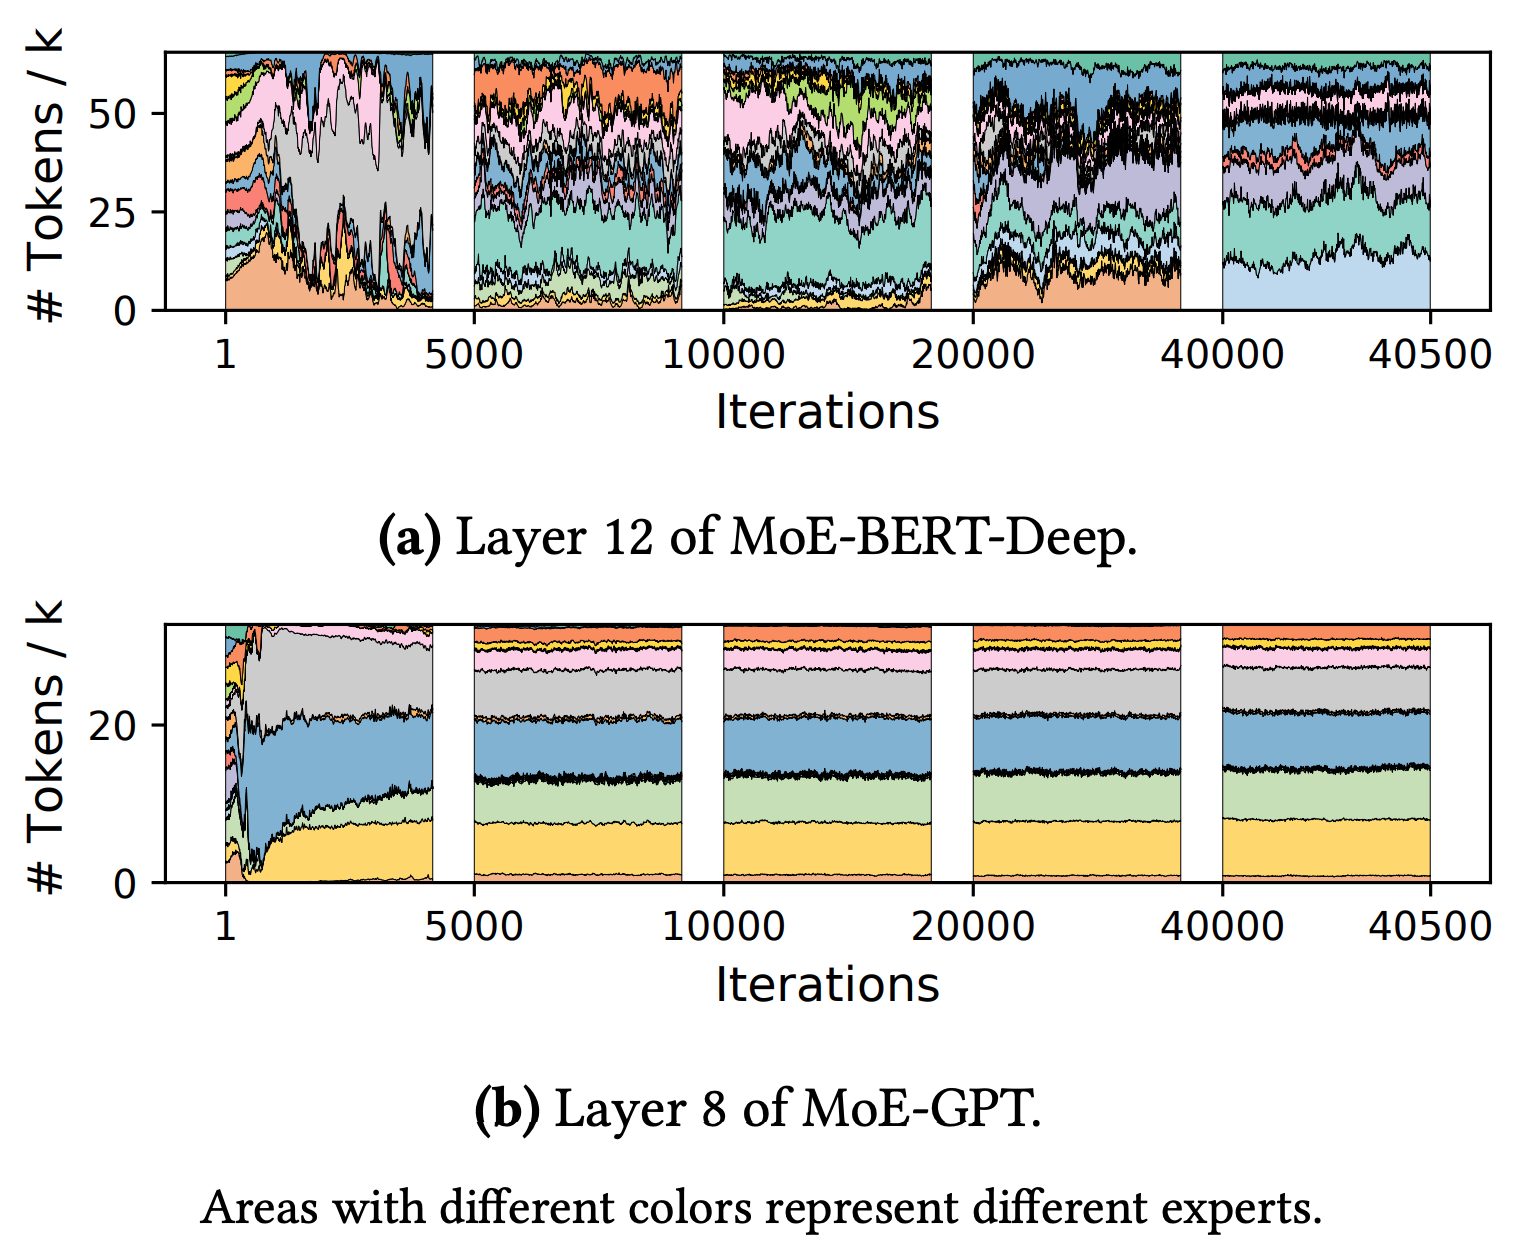
\includegraphics[width=0.6\linewidth]{figures/experts_popularity.png}
    \caption{\textbf{Load balance among experts across iterations~\cite{fastermoe}} Two models show different patterns of expert popularity over the course of training with the FasterMoE framework }
    \label{fig:expert_popularity}
\end{figure}

\subsubsection{Architecture}

A Mixture-of-Experts (MoE) layer can be defined as follows~\cite{shazeer2017}:
\begin{equation}
    y = \sum_i^n G(x)_i E_i(x)
\end{equation}

where $E_i$ is the $i$-th expert and $G(x)$ is a gating network returning a sparse $n$-dimensional vector. There can be thousands of experts, but whenever $G(X)_i=0$, we don't have to compute $E_i(x)$, since it won't be a factor in the output.

%If the number of experts is very large, we can build a two-level hierarchical MoE, and reduce the branching factor~\cite{shazeer2017}: 
%\begin{equation}
%y_H = \sum_{i=1}^a \sum_{j=1}^b G_{\text{primary}}(x)_i \cdot G_i(x)_j \cdot E_{i,j}(x)
%\end{equation}
%where we are selecting among $a$ groups of $b$ experts each by means of a primary gating network $G_{\text{primary}}$ and $a$ secondary gating networks. 

An important parameter in MoE architectures is the \textit{expert capacity}, or the batch size of each expert (the maximum number of tokens than can routed to an expert). A commonly-used formula~\cite{tutel} for the expert capacity is shown in Equation \ref{eq:expert_capacity}, where $k$ is the parameter from the top-k gating function, $T$ is the number of tokens per batch, $E$ is the number of experts, and $f$ is the \textit{capacity factor}.
\begin{equation}\label{eq:expert_capacity}
    expert\_capacity = k \cdot f \cdot \frac{T}{E}
\end{equation}
The expert capacity is usually tuned through the capacity factor, and allows us to trade between the likelihood of expert overflow (when the number of token dispatched to an expert exceeds the expert capacity) and greater computation and communication costs \cite{switch_transformer}. 


%\subsection{Token Routing}
%\subsection{Load Balancing}
%\subsection{Communication costs optimization }



\subsection{GPT-MoE}\label{gpt-moe}
The GPT model can be easily \textit{MoEfied} by substituting the feed forward network in the decoder with a MoE layer. For example, the sparse models~\cite{fairseq-checkpoint} whose checkpoints are available in the Fairseq repository~\footnote{\url{https://github.com/facebookresearch/fairseq/tree/main/examples/moe_lm}} use 12 (15B-parameters model), 24 (52B- parameters and 207B-parameters models) or 32 (1.1T-parameters model) decoder layers, where every other layer contains a MoE component instead of the regular FFN. In Listing \ref{fairseq-15-moe}, we can see the 15B parameters model, where the six even-numbered decoder layers contain a FFN with two fully-connected layers, and the six odd-numbered decoder layers contain a MoE Layer instead.

\begin{lstlisting}[caption=Fairseq’s 15B-parameters MoE model, breaklines=true, basicstyle=\footnotesize, frame=single, label=fairseq-15-moe]
TransformerLanguageModel(
  (decoder): TransformerDecoder(
    (dropout_module): FairseqDropout(p=0.1)
    (embed_tokens): Embedding(50264, 768, padding_idx=1)
    (embed_positions): SinusoidalPositionalEmbedding()
    (layers): ModuleList(
      (0): TransformerDecoderLayer(
        [checkpointed]
        (dropout_module): FairseqDropout(p=0.1)
        (self_attn): MultiheadAttention(
          (dropout_module): FairseqDropout(p=0.1)
          (k_proj): Linear(in_features=768, out_features=768, bias=True)
          (v_proj): Linear(in_features=768, out_features=768, bias=True)
          (q_proj): Linear(in_features=768, out_features=768, bias=True)
          (out_proj): Linear(in_features=768, out_features=768, bias=True)
        )
        (self_attn_layer_norm): LayerNorm((768,), eps=1e-05, elementwise_affine=True)
        (activation_dropout_module): FairseqDropout(p=0.0)
        (fc1): Linear(in_features=768, out_features=3072, bias=True)
        (fc2): Linear(in_features=3072, out_features=768, bias=True)
        (final_layer_norm): LayerNorm((768,), eps=1e-05, elementwise_affine=True)
      )
      (1): TransformerDecoderLayer(
        [checkpointed]
        (dropout_module): FairseqDropout(p=0.1)
        (self_attn): MultiheadAttention(
          (dropout_module): FairseqDropout(p=0.1)
          (k_proj): Linear(in_features=768, out_features=768, bias=True)
          (v_proj): Linear(in_features=768, out_features=768, bias=True)
          (q_proj): Linear(in_features=768, out_features=768, bias=True)
          (out_proj): Linear(in_features=768, out_features=768, bias=True)
        )
        (self_attn_layer_norm): LayerNorm((768,), eps=1e-05, elementwise_affine=True)
        (moe_layer): MOELayer()
        (final_layer_norm): LayerNorm((768,), eps=1e-05, elementwise_affine=True)
      )

      ...
      
      
      (11): TransformerDecoderLayer(
        [checkpointed]
        (dropout_module): FairseqDropout(p=0.1)
        (self_attn): MultiheadAttention(
          (dropout_module): FairseqDropout(p=0.1)
          (k_proj): Linear(in_features=768, out_features=768, bias=True)
          (v_proj): Linear(in_features=768, out_features=768, bias=True)
          (q_proj): Linear(in_features=768, out_features=768, bias=True)
          (out_proj): Linear(in_features=768, out_features=768, bias=True)
        )
        (self_attn_layer_norm): LayerNorm((768,), eps=1e-05, elementwise_affine=True)
        (moe_layer): MOELayer()
        (final_layer_norm): LayerNorm((768,), eps=1e-05, elementwise_affine=True)
      )
    )
    (layer_norm): LayerNorm((768,), eps=1e-05, elementwise_affine=True)
    (output_projection): Linear(in_features=768, out_features=50264, bias=False)
  )
)
\end{lstlisting}


\section{Related Works}\label{related-works}
In this section, we introduce existing serving systems for Transformers/GPT (Section \ref{transformer-serving}) and GPT-MoE (Section \ref{chpt2-moe-serving}) models.

\subsection{Transformer serving systems}\label{transformer-serving}
There is a large number of systems that can serve transformers. In this section, we focus on the systems that are specifically optimized for transformers. These systems are also the ones that have more similar components to ExpertFlow.

\subsubsection{TurboTransformers}
TurboTransformer~\cite{turbo_transformers} is an inference system for transformers from Tencent. The system consists of two components (see Figure \ref{fig:turbo-transformers}): a serving framework, and a computational runtime.

\begin{figure}[H]
    \centering
    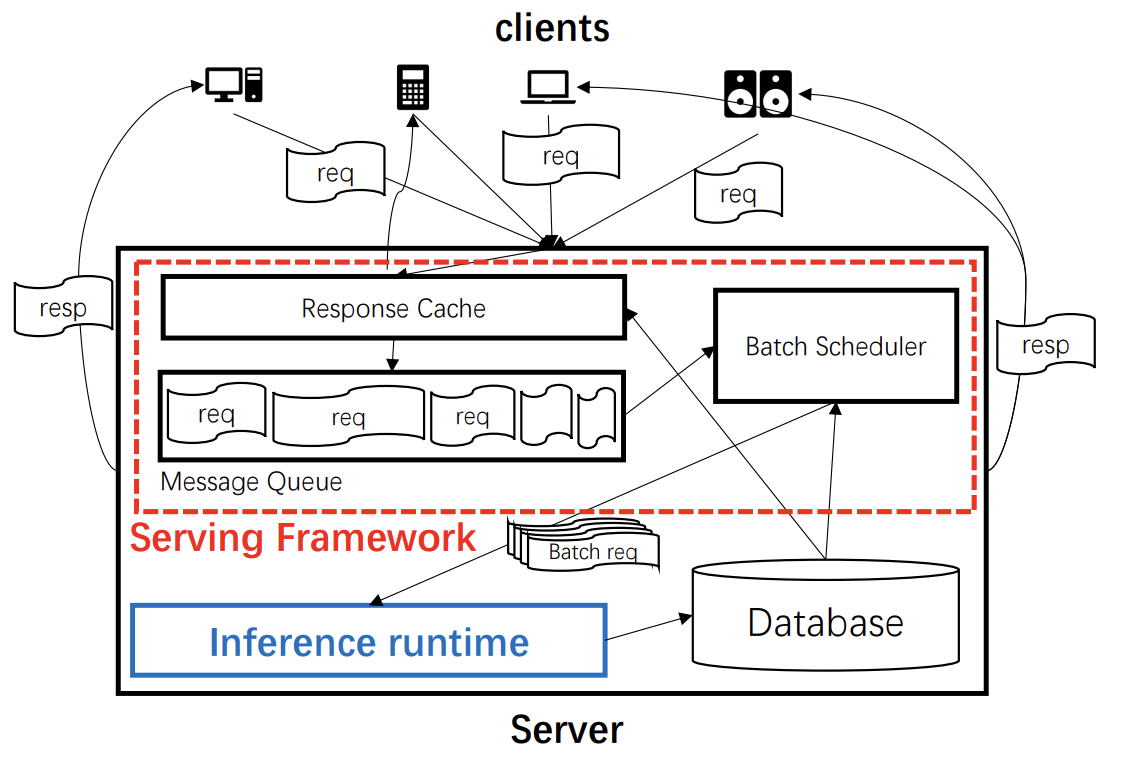
\includegraphics[width=0.6\linewidth]{figures/turbo_transformers.png}
    \caption{\textbf{The TurboTransformers system} A diagram~\cite{fastermoe} showing the components of the TurboTransformers system}
    \label{fig:turbo-transformers}
\end{figure}

The serving framework receives requests from the user via a gRPC/HTTP endpoint, and uses a dynamic programming algorithm to decide how to batch together the requests that arrive over a specific interval of time. The batch assignment considers the length of each request and attempts to minimize the amount of padding needed while also maximizing the performance gains that come from batching together as many requests as possible. 

The computational runtime takes the DNN model as input, represents it as a computational graph, and fuses all the non-GEMM kernels together. The fused computations are implemented with custom CUDA kernels that come with the TurboTransformers framework. In particular, the framework focuses on optimizing the performance of reduction kernels, such as those needed in the Softmax and LayerNorm operators. In addition to the kernel optimizations, the computational runtime also includes a custom memory manager to minimize the GPU memory overhead by reusing as much allocated memory as possible to store intermediate results. This is made possible thanks to a memory allocator that takes into consideration the topology of the computational graph to decide when to assign different tensors to the same region in memory.

The main limitations of the TurboTransformers system are the lack of support for the MoE architecture, and more importantly, the lack of support for multi-GPU and multi-node machines.


\subsubsection{FasterTransformer and Triton}
FasterTransformer~\cite{faster_transformer} (FT) is an open-source inference system by NVIDIA supporting multi-GPU execution. As the name suggests, the inference system is specialized for Transformers, and it supports a wide variety of models, including BERT~\cite{bert}, XLNet~\cite{xlnet}, GPT~\cite{gpt1, gpt2, brown_2020}, OPT~\cite{opt}, GPT-MoE, BLOOM~\cite{bloom}, GPT-J~\cite{gpt-j}, Longformer~\cite{longformer}, T5~\cite{t5}, Swin Transformer~\cite{swin-transformer}, and ViT~\cite{vit}. The FasterTransformer's backend is implemented using C++, CUDA and cuBLAS, and several front-ends are available, including C++, TensorFlow and PyTorch. The repository contains an example MoE implementation~\footnote{\url{https://github.com/NVIDIA/FasterTransformer/blob/main/docs/gpt\_guide.md\#gpt-with-moe}}, which we use in our evaluation to compare the performance of ExpertFlow with FT. 

Unlike TurboTransformers, FasterTransformer does not come with a serving framework, but NVIDIA released Triton~\cite{triton}, an open-source inference system that can be coupled with FasterTransformer via the Triton FasterTransformer Backend~\cite{triton-ft-backend}.

\subsubsection{Orca}
Orca~\cite{orca} is a distributed inference system for transformers, employing optimizations such as dynamic batching and iteration-level scheduling to boost the performance of variable-length requests whose arrival times are not known in advance. Unfortunately, the Orca code is closed-source, and the authors are not planning to make it publicly available as it is being used in production by for-profit company FriendliAI, so we cannot compare the performance with our system. 

\subsection{Speculative decoding systems}
Two speculative decoding systems~\cite{speculative-decoding-berkeley, speculative-decoding-google} have been introduced in recent months. The main difference between these systems and ExpertFlow is that the former ones only support the use of a single \textit{speculator} (i.e. a single small model), which may not align well with the larger target model because of the gap in the number of parameters between the smaller and larger model. On the other hand, ExpertFlow supports the use of a combination of boost-tuned smaller models, which greatly improve the quality of the speculated tokens.

\section{MoE Serving Systems}\label{chpt2-moe-serving}
There are several distributed inference systems that are capable of serving MoE models. For example, FasterTransformer mentioned above, together with Fairseq~\cite{fairseq} (with additional support for the Tutel~\cite{tutel} optimizations) and Alpa~\cite{alpa}. These systems, however, were designed primarily for training and do not have as many optimizations as DeepSpeed-MoE~\cite{deepspeed-moe} for the MoE inference scenario.

\subsection{DeepSpeed-MoE}
DeepSpeed-MoE~\cite{deepspeed-moe} is currently the most well-optimized distributed inference framework with best performance for serving MoE models. The optimizations behind DeepSpeed-MoE's performance can be divided in three categories: the parallelization plan (see Figure \ref{fig:deepspeed-moe-parallelization}), the hierarchical all-to-all communications (see Figure \ref{fig:deepspeed-moe-a2a}), and the use of an efficient kernel for the MoE layers.
\begin{figure}[H]
    \centering
    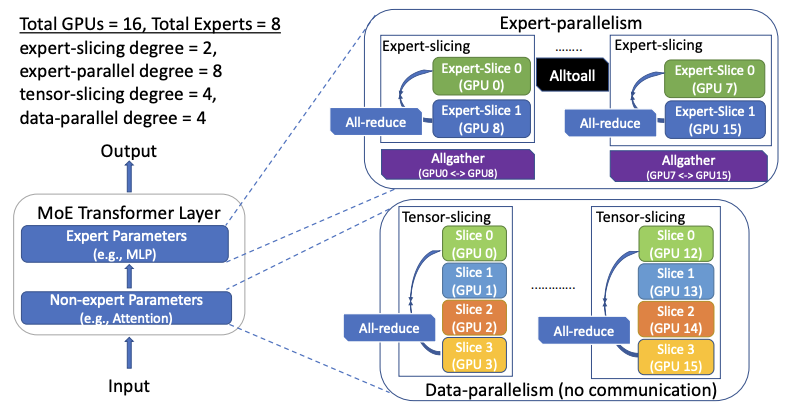
\includegraphics[width=0.6\linewidth]{figures/deepspeed-moe-parallelization.png}
    \caption{\textbf{The DeepSpeed-MoE parallelization mechanism~\cite{deepspeed-moe}}}
    \label{fig:deepspeed-moe-parallelization}
\end{figure}
\begin{figure}[H]
    \centering
    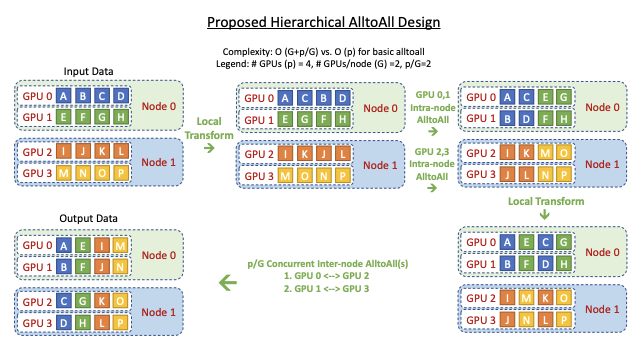
\includegraphics[width=0.6\linewidth]{figures/deepspeed-moe-a2a.png}
    \caption{\textbf{The DeepSpeed-MoE Hierarchical all-to-all design~\cite{deepspeed-moe}}}
    \label{fig:deepspeed-moe-a2a}
\end{figure}
DeepSpeed-MoE's parallelization plan consists of a combination of data, model and expert parallelism. Figure \ref{fig:deepspeed-moe-parallelization} shows how a GPT-MoE model will be parallelized on a machine with 16 GPUs. In each MoE layer, experts are divided in 8 blocks (\texttt{expert parallel degree = 8}), and the tensor containing the parameters for each expert block is partitioned across 2 GPUs (\texttt{expert slicing degree = 2}). The tensors containing the parameters from the non-MoE layers are split across 4 GPUs (\texttt{tensor slicing degree = 4}), and they are replicated 4 times (\texttt{data parallel degree = 4}).
